\chapter{Mathematical Foundations For TinyGPT}

Chapter 1 showed the whole TinyGPT pipeline. This chapter slows down and builds the mathematical tools behind that pipeline. The purpose is not abstract mathematics for its own sake. Every symbol in this chapter will be connected to the TinyGPT sample case, to tensor shapes, and to source-code operations.

\section{Chapter Goals}

By the end of this chapter, you should be able to:

\begin{itemize}
  \item distinguish scalars, vectors, matrices, and tensors in a GPT model;
  \item map TinyGPT token data to mathematical shapes;
  \item explain matrix multiplication as the core operation inside linear layers;
  \item compute softmax and cross-entropy loss for one TinyGPT prediction;
  \item explain gradients as directions for changing model parameters;
  \item read simple source-code functions for linear layers, softmax, loss, and gradient updates.
\end{itemize}

\section{The Running TinyGPT Example}

We keep the same sample sentence:

\begin{quote}
\texttt{Tiny GPT models learn from tokens .}
\end{quote}

Using the Chapter 1 vocabulary, this becomes:

\[
[2,3,4,5,6,7,8].
\]

With context length \(T=4\), one input-target pair is:

\[
x=[2,3,4,5],
\qquad
y=[3,4,5,6].
\]

In this chapter, we use the toy dimensions:

\[
B=2,\qquad T=4,\qquad C=6,\qquad V=9.
\]

\begin{longtable}{p{0.18\textwidth}p{0.24\textwidth}p{0.44\textwidth}}
\toprule
\term{Symbol} & \term{TinyGPT value} & \term{Meaning} \\
\midrule
\(B\) & 2 & two examples per batch \\
\(T\) & 4 & four token positions per example \\
\(C\) & 6 & six numbers per embedding vector \\
\(V\) & 9 & nine possible vocabulary tokens \\
\(x\) & \([2,3,4,5]\) & input token IDs \\
\(y\) & \([3,4,5,6]\) & target next-token IDs \\
\bottomrule
\end{longtable}

\section{How Math Objects Are Managed In Software}

Mathematical objects become named tensors and parameters in source code. A beginner should learn to ask three questions about every object:

\begin{enumerate}
  \item \term{What is it?} A scalar, vector, matrix, or tensor.
  \item \term{Who owns it?} Data loader, model, loss function, optimizer, or checkpoint.
  \item \term{How does it change?} Fixed input, trainable parameter, intermediate activation, gradient, or logged result.
\end{enumerate}

\begin{center}
\begin{tikzpicture}[
  box/.style={draw, rounded corners=2pt, minimum height=0.72cm, text width=2.45cm, align=center},
  arrow/.style={-{Latex[length=2mm]}, thick},
  lab/.style={font=\small, align=center}
]
\node[box, fill=blue!5] (x) at (0,0) {\(x\)\\input IDs\\fixed batch};
\node[box, fill=blue!5] (theta) at (3.0,0) {\(\theta\)\\parameters\\trainable};
\node[box, fill=red!8] (act) at (6.0,0) {activations\\hidden tensors\\temporary};
\node[box, fill=red!8] (loss) at (9.0,0) {\(L\)\\loss\\scalar result};
\node[box, fill=gray!12] (grad) at (6.0,-1.45) {\(\nabla_\theta L\)\\gradients\\computed};
\node[box, fill=gray!12] (opt) at (3.0,-1.45) {optimizer state\\AdamW moments\\updated};
\draw[arrow] (x) -- (act);
\draw[arrow] (theta) -- (act);
\draw[arrow] (act) -- (loss);
\draw[arrow] (loss) -- (grad);
\draw[arrow] (grad) -- (opt);
\draw[arrow] (opt) -- (theta);
\node[lab] at (4.6,-2.35) {Forward pass creates activations and loss. Backward pass creates gradients. Optimizer updates parameters.};
\end{tikzpicture}
\end{center}

\begin{longtable}{p{0.18\textwidth}p{0.22\textwidth}p{0.22\textwidth}p{0.24\textwidth}}
\toprule
\term{Object} & \term{TinyGPT shape} & \term{Owner} & \term{Stored in checkpoint?} \\
\midrule
Token IDs \(x\) & \shape{[B,T]} & data loader & no \\
Targets \(y\) & \shape{[B,T]} & data loader & no \\
Embeddings & \shape{[V,C]} & model & yes \\
Activations & \shape{[B,T,C]} & forward pass & usually no \\
Logits & \shape{[B,T,V]} & model output & no \\
Loss \(L\) & scalar & loss function & logged, not as weight \\
Gradients & same as parameters & autograd & no \\
Optimizer state & parameter-shaped & optimizer & yes for resume \\
\bottomrule
\end{longtable}

This is the real operational logic behind the math. The equation \(f_\theta(x)=Z\) is not just notation: \(x\) comes from the data loader, \(\theta\) lives inside the model, \(Z\) is a temporary output, and the loss turns \(Z\) into a training signal.

\section{Scalars: One Number With One Meaning}

A \term{scalar} is a single number. In TinyGPT, examples include:

\begin{itemize}
  \item one loss value, such as \(L=0.446\);
  \item one learning rate, such as \(\eta=0.001\);
  \item one logit score for one token, such as \(z_7=2.2\);
  \item one probability, such as \(p_7=0.64\).
\end{itemize}

The important habit is to attach meaning to the number. The scalar \(0.64\) is not just a number. In our running example it may mean:

\[
p_{\texttt{tokens}} = 0.64,
\]

the model's probability for token ID \(7\), \texttt{tokens}, after seeing the context \texttt{Tiny GPT models learn from}.

\begin{center}
\begin{tikzpicture}[
  box/.style={draw, rounded corners=2pt, minimum height=0.65cm, text width=2.4cm, align=center},
  arrow/.style={-{Latex[length=2mm]}, thick}
]
\node[box, fill=blue!5] (context) at (0,0) {\texttt{Tiny GPT}\\\texttt{models learn from}};
\node[box, fill=red!8] (prob) at (3.5,0) {\(p_7=0.64\)\\for \texttt{tokens}};
\draw[arrow] (context) -- (prob);
\end{tikzpicture}
\end{center}

\section{Vectors: One Token Becomes A List Of Features}

A \term{vector} is an ordered list of numbers:

\[
\mathbf{v} =
\begin{bmatrix}
v_1\\v_2\\v_3\\v_4\\v_5\\v_6
\end{bmatrix}
\in \mathbb{R}^{6}.
\]

In TinyGPT, the token \texttt{Tiny} has token ID \(2\). The embedding table maps ID \(2\) to a vector of length \(C=6\):

\[
E_{\text{tok}}[2] =
\begin{bmatrix}
0.12\\
-0.04\\
0.31\\
0.08\\
-0.17\\
0.22
\end{bmatrix}.
\]

These numbers are examples, not fixed facts. At initialization they are random. During training, they change.

\begin{center}
\begin{tikzpicture}[
  cell/.style={draw, minimum width=0.72cm, minimum height=0.52cm, align=center},
  box/.style={draw, rounded corners=2pt, minimum width=1.1cm, minimum height=0.65cm, align=center},
  arrow/.style={-{Latex[length=2mm]}, thick}
]
\node[box, fill=blue!5] (id) at (0,0) {ID 2\\\texttt{Tiny}};
\node[box] (row) at (2.0,0) {embedding\\row 2};
\foreach \i/\v in {0/0.12,1/-0.04,2/0.31,3/0.08,4/-0.17,5/0.22} {
  \node[cell, fill=red!5] at (3.75+\i*0.78,0) {\scriptsize \v};
}
\draw[arrow] (id) -- (row);
\draw[arrow] (row) -- (3.35,0);
\node[font=\small] at (5.7,-0.75) {a vector in \(\mathbb{R}^{6}\)};
\end{tikzpicture}
\end{center}

\term{Code logic}: an embedding lookup is an index operation.

\begin{lstlisting}[language=Python]
embedding_table = torch.randn(vocab_size, n_embd)  # [V, C]
tiny_vector = embedding_table[2]                   # [C]
\end{lstlisting}

\term{Why it works}: token IDs are discrete symbols. Vectors are numerical objects that can be added, multiplied, compared, and updated by gradient descent.

\section{Matrices: Tables That Transform Vectors}

A \term{matrix} is a rectangular array of numbers:

\[
W \in \mathbb{R}^{C \times V}.
\]

In TinyGPT, the language-model head maps a hidden vector of length \(C=6\) to vocabulary logits of length \(V=9\):

\[
\mathbf{z} = \mathbf{h} W_{\text{out}} + \mathbf{b}.
\]

The shapes are:

\[
\mathbf{h} \in \mathbb{R}^{1 \times 6},
\qquad
W_{\text{out}} \in \mathbb{R}^{6 \times 9},
\qquad
\mathbf{z} \in \mathbb{R}^{1 \times 9}.
\]

\begin{center}
\begin{tikzpicture}[
  box/.style={draw, rounded corners=2pt, minimum height=0.75cm, text width=2.1cm, align=center},
  arrow/.style={-{Latex[length=2mm]}, thick}
]
\node[box, fill=blue!5] (h) at (0,0) {hidden vector\\\shape{[1,6]}};
\node[box, fill=blue!5] (w) at (3.0,0) {output matrix\\\shape{[6,9]}};
\node[box, fill=red!8] (z) at (6.0,0) {logits\\\shape{[1,9]}};
\draw[arrow] (h) -- node[above] {\(\times\)} (w);
\draw[arrow] (w) -- (z);
\end{tikzpicture}
\end{center}

This is a linear layer. In PyTorch:

\begin{lstlisting}[language=Python]
lm_head = torch.nn.Linear(6, 9)
z = lm_head(h)  # h: [1, 6], z: [1, 9]
\end{lstlisting}

\section{Tensors: Batches Of Structured Numbers}

A \term{tensor} is a multidimensional array. GPT training uses tensors constantly:

\begin{lstlisting}
input ids:          [B, T]
embeddings:         [B, T, C]
attention scores:   [B, H, T, T]
logits:             [B, T, V]
targets:            [B, T]
\end{lstlisting}

For TinyGPT:

\[
x \in \mathbb{Z}^{2 \times 4},
\qquad
X \in \mathbb{R}^{2 \times 4 \times 6},
\qquad
Z \in \mathbb{R}^{2 \times 4 \times 9}.
\]

\begin{center}
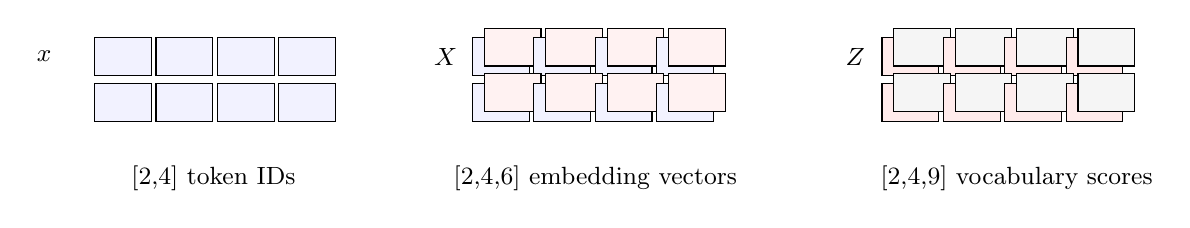
\begin{tikzpicture}[
  cell/.style={draw, minimum width=0.72cm, minimum height=0.48cm, align=center},
  lab/.style={font=\small}
]
\node[lab] at (-1.0,0) {\(x\)};
\foreach \r in {0,1} {
  \foreach \c in {0,1,2,3} {
    \node[cell, fill=blue!5] at (\c*0.78,-\r*0.58) {};
  }
}
\node[lab] at (1.15,-1.55) {\shape{[2,4]} token IDs};
\node[lab] at (4.1,0) {\(X\)};
\foreach \r in {0,1} {
  \foreach \c in {0,1,2,3} {
    \node[cell, fill=blue!5] at (4.8+\c*0.78,-\r*0.58) {};
    \node[cell, fill=red!5] at (4.95+\c*0.78,-\r*0.58+0.12) {};
  }
}
\node[lab] at (6.0,-1.55) {\shape{[2,4,6]} embedding vectors};
\node[lab] at (9.3,0) {\(Z\)};
\foreach \r in {0,1} {
  \foreach \c in {0,1,2,3} {
    \node[cell, fill=red!8] at (10.0+\c*0.78,-\r*0.58) {};
    \node[cell, fill=gray!8] at (10.15+\c*0.78,-\r*0.58+0.12) {};
  }
}
\node[lab] at (11.35,-1.55) {\shape{[2,4,9]} vocabulary scores};
\end{tikzpicture}
\end{center}

\term{Why tensors matter}: one training step should process many examples and many positions efficiently. Tensors let the code ask the GPU to perform many operations at once.

\section{Visual Tensor Geometry}

Students often understand tensors faster when they stop imagining them as mysterious objects and start seeing them as stacked tables. A tensor is an array with axes. Each axis has a meaning.

\subsection{A Rank-2 Tensor: Token IDs}

The input token tensor has shape \shape{[B,T]}. For TinyGPT, \shape{[2,4]} means two rows and four columns:

\begin{center}
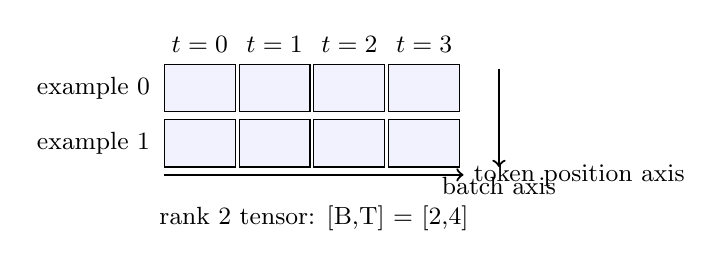
\begin{tikzpicture}[
  cell/.style={draw, minimum width=0.9cm, minimum height=0.6cm, align=center},
  lab/.style={font=\small}
]
\foreach \r/\name in {0/example 0,1/example 1} {
  \node[lab, align=right] at (-1.35,-\r*0.7) {\name};
}
\foreach \c in {0,1,2,3} {
  \node[lab] at (\c*0.95,0.55) {\(t=\c\)};
}
\foreach \r/\vals in {0/{2,3,4,5},1/{0,1,2,3}} {
  \foreach \c in {0,1,2,3} {
    \node[cell, fill=blue!5] at (\c*0.95,-\r*0.7) {};
  }
}
\node[lab] at (1.45,-1.65) {rank 2 tensor: \shape{[B,T]} = \shape{[2,4]}};
\draw[->, thick] (-0.45,-1.1) -- (3.35,-1.1) node[right] {\small token position axis};
\draw[->, thick] (3.8,0.25) -- (3.8,-1.0) node[below] {\small batch axis};
\end{tikzpicture}
\end{center}

Each cell is one integer token ID. This tensor is not yet a language representation; it is an index grid.

\subsection{A Rank-3 Tensor: Embeddings}

After embedding lookup, every token ID becomes a vector of length \(C=6\). The shape becomes \shape{[B,T,C]} = \shape{[2,4,6]}. You can visualize this as a small box: batch axis, position axis, and channel axis.

\begin{center}
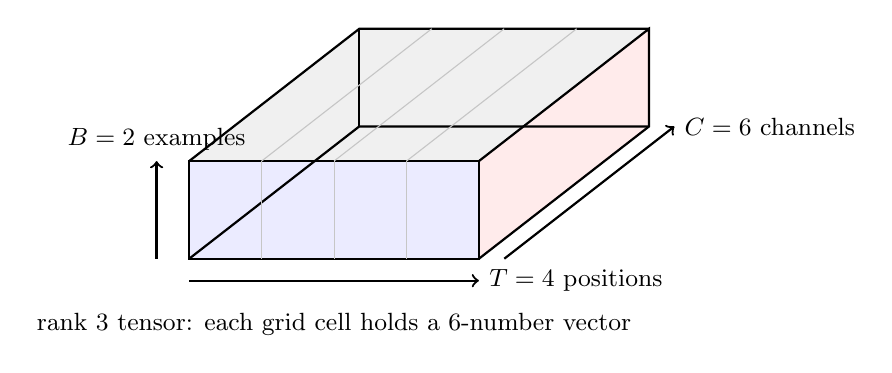
\begin{tikzpicture}[
  x={(0.92cm,0cm)},
  y={(0cm,0.62cm)},
  z={(0.36cm,0.28cm)},
  lab/.style={font=\small}
]
\coordinate (O) at (0,0,0);
\coordinate (X) at (4,0,0);
\coordinate (Y) at (0,2,0);
\coordinate (Z) at (0,0,6);
\coordinate (XY) at (4,2,0);
\coordinate (XZ) at (4,0,6);
\coordinate (YZ) at (0,2,6);
\coordinate (XYZ) at (4,2,6);

\fill[blue!8] (O) -- (X) -- (XY) -- (Y) -- cycle;
\fill[red!8] (X) -- (XZ) -- (XYZ) -- (XY) -- cycle;
\fill[gray!12] (Y) -- (XY) -- (XYZ) -- (YZ) -- cycle;
\draw[thick] (O) -- (X) -- (XY) -- (Y) -- cycle;
\draw[thick] (X) -- (XZ) -- (XYZ) -- (XY);
\draw[thick] (Y) -- (YZ) -- (XYZ);
\draw[thick] (O) -- (Z) -- (XZ);
\draw[thick] (Z) -- (YZ);

\foreach \i in {1,2,3} {
  \draw[gray!45] (\i,0,0) -- (\i,2,0);
  \draw[gray!45] (\i,2,0) -- (\i,2,6);
}
\draw[->, thick] (0,-0.45,0) -- (4,-0.45,0) node[right] {\small \(T=4\) positions};
\draw[->, thick] (-0.45,0,0) -- (-0.45,2,0) node[above] {\small \(B=2\) examples};
\draw[->, thick] (4.35,0,0) -- (4.35,0,6) node[right] {\small \(C=6\) channels};
\node[lab, align=center] at (2,-1.35,0) {rank 3 tensor: each grid cell holds a 6-number vector};
\end{tikzpicture}
\end{center}

The channel axis is where learned features live. A single position, such as token \texttt{Tiny} in example 0, is one vector:

\[
X_{0,0,:}\in\mathbb{R}^{6}.
\]

The colon means ``take all entries along this axis.'' In code:

\begin{lstlisting}[language=Python]
one_vector = X[0, 0, :]  # [C] = [6]
\end{lstlisting}

\subsection{Slices: How To Read Tensor Indexing}

Tensor indexing is easier if you think of slicing a block.

\begin{center}
\begin{tikzpicture}[
  cell/.style={draw, minimum width=0.8cm, minimum height=0.48cm, align=center},
  lab/.style={font=\small, align=center},
  arrow/.style={-{Latex[length=2mm]}, thick}
]
\node[lab] at (0,1.0) {embedded tensor \(X\): \shape{[2,4,6]}};
\foreach \r in {0,1} {
  \foreach \c in {0,1,2,3} {
    \node[cell, fill=blue!5] at (\c*0.82,-\r*0.55) {};
  }
}
\draw[red, very thick] (-0.4,0.3) rectangle (3.05,-0.25);
\node[lab, text=red!70!black] at (4.7,0.0) {\(X[0,:,:]\): all positions\\for example 0, shape \shape{[4,6]}};
\draw[arrow, red!70!black] (3.1,0.0) -- (3.8,0.0);

\foreach \r in {0,1} {
  \foreach \c in {0,1,2,3} {
    \node[cell, fill=blue!5] at (\c*0.82,-2.2-\r*0.55) {};
  }
}
\draw[maplered, very thick] (1.25,-3.05) rectangle (2.0,-1.9);
\node[lab, text=maplered] at (4.85,-2.5) {\(X[:,2,:]\): position 2\\from every example, shape \shape{[2,6]}};
\draw[arrow, maplered] (2.05,-2.5) -- (3.65,-2.5);
\end{tikzpicture}
\end{center}

\begin{longtable}{p{0.24\textwidth}p{0.26\textwidth}p{0.34\textwidth}}
\toprule
\term{Slice} & \term{Shape} & \term{Meaning} \\
\midrule
\texttt{X[0,0,:]} & \shape{[6]} & one token vector \\
\texttt{X[0,:,:]} & \shape{[4,6]} & all positions in example 0 \\
\texttt{X[:,2,:]} & \shape{[2,6]} & position 2 from every example \\
\texttt{X[:,:,3]} & \shape{[2,4]} & channel 3 across batch and positions \\
\bottomrule
\end{longtable}

\subsection{Broadcasting: Adding Position Embeddings}

TinyGPT combines token identity and position by adding token embeddings and position embeddings:

\[
X = E_{\text{tok}}(x) + E_{\text{pos}}(0:T-1).
\]

The shapes are:

\[
\shape{[B,T,C]} + \shape{[T,C]} \rightarrow \shape{[B,T,C]}.
\]

The position matrix \shape{[T,C]} is reused for every batch row. This is called broadcasting.

\begin{center}
\begin{tikzpicture}[
  box/.style={draw, rounded corners=2pt, minimum height=0.75cm, text width=2.2cm, align=center},
  arrow/.style={-{Latex[length=2mm]}, thick},
  lab/.style={font=\small}
]
\node[box, fill=blue!5] (tok) at (0,0) {token embeddings\\\shape{[2,4,6]}};
\node[box, fill=red!8] (pos) at (0,-1.3) {position embeddings\\\shape{[4,6]}};
\node[box, fill=gray!10] (sum) at (4.0,-0.65) {initial hidden state\\\shape{[2,4,6]}};
\draw[arrow] (tok.east) -- (sum.west);
\draw[arrow] (pos.east) -- (sum.west);
\node[lab, align=center] at (2.0,-1.95) {same position vectors are added\\to every example in the batch};
\end{tikzpicture}
\end{center}

\term{Code logic}:

\begin{lstlisting}[language=Python]
tok = token_emb(idx)       # [B, T, C]
pos = pos_emb(positions)   # [T, C]
x = tok + pos              # [B, T, C], broadcast over B
\end{lstlisting}

\subsection{Rank-4 Tensors: Attention Scores}

Attention introduces a rank-4 tensor. If TinyGPT has \(H=2\) heads, attention scores have shape:

\[
\shape{[B,H,T,T]} = \shape{[2,2,4,4]}.
\]

The axes mean:

\begin{itemize}
  \item \(B\): which example in the batch;
  \item \(H\): which attention head;
  \item first \(T\): which position is reading;
  \item second \(T\): which position is being read.
\end{itemize}

\begin{center}
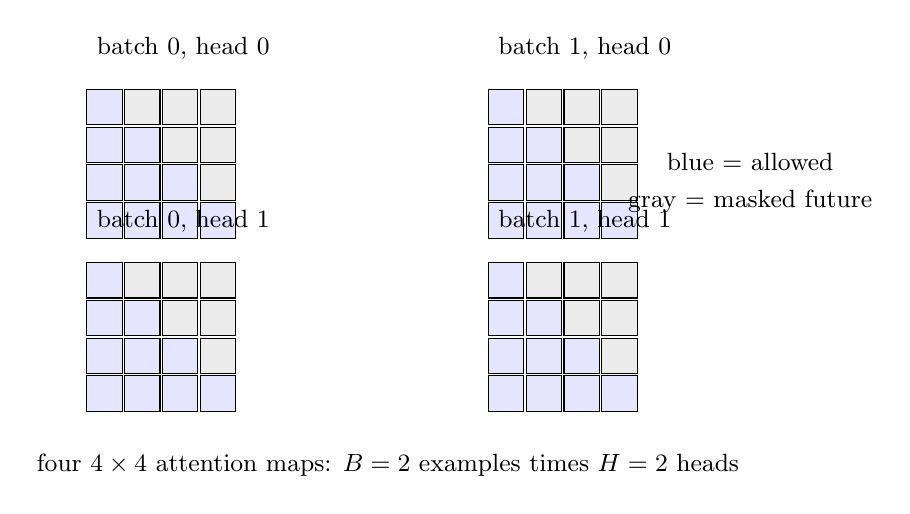
\begin{tikzpicture}[
  cell/.style={draw, minimum width=0.45cm, minimum height=0.45cm},
  lab/.style={font=\small}
]
\foreach \b/\xshift in {0/0,1/5.1} {
  \foreach \h/\yshift in {0/0,1/-2.2} {
    \node[lab] at (\xshift+1.0,\yshift+0.75) {batch \(\b\), head \(\h\)};
    \foreach \r in {0,1,2,3} {
      \foreach \c in {0,1,2,3} {
        \ifnum\c>\r
          \node[cell, fill=gray!15] at (\xshift+\c*0.48,\yshift-\r*0.48) {};
        \else
          \node[cell, fill=blue!10] at (\xshift+\c*0.48,\yshift-\r*0.48) {};
        \fi
      }
    }
  }
}
\node[lab, align=center] at (3.6,-4.55) {four \(4\times4\) attention maps: \(B=2\) examples times \(H=2\) heads};
\node[lab] at (8.2,-0.7) {blue = allowed};
\node[lab] at (8.2,-1.2) {gray = masked future};
\end{tikzpicture}
\end{center}

This diagram is the visual logic of causal attention. Each head has a table saying how much each position reads from each previous position.

\section{Preview: Context Vectors As Weighted Sums}

Attention will receive a full chapter later, but the core visual idea is useful now.
A context vector is a weighted combination of input vectors. This first arithmetic
example is \emph{unmasked} attention, not TinyGPT's causal forward pass: the second
position reads future positions too. Causal attention must instead set
\(\alpha_{23}=\alpha_{24}=0\) and renormalize the allowed weights.

Suppose TinyGPT has four token vectors:

\[
x^{(1)}=\texttt{Tiny},\quad
x^{(2)}=\texttt{GPT},\quad
x^{(3)}=\texttt{models},\quad
x^{(4)}=\texttt{learn}.
\]

To build a context vector for the second position, \(z^{(2)}\), attention computes:

\[
z^{(2)} =
\alpha_{21}x^{(1)}
+ \alpha_{22}x^{(2)}
+ \alpha_{23}x^{(3)}
+ \alpha_{24}x^{(4)}.
\]

The weights satisfy:

\[
\alpha_{21}+\alpha_{22}+\alpha_{23}+\alpha_{24}=1.
\]

\begin{center}
\begin{tikzpicture}[
  vec/.style={draw, minimum width=0.52cm, minimum height=0.48cm, align=center},
  word/.style={font=\small, align=center},
  arrow/.style={-{Latex[length=2mm]}, thick},
  lab/.style={font=\small, align=center}
]
\foreach \i/\tok/\a/\b/\c in {0/Tiny/0.2/0.4/0.1,1/GPT/0.5/0.1/0.3,2/models/0.4/0.7/0.2,3/learn/0.1/0.3/0.8} {
  \node[word] at (\i*2.15,1.25) {\texttt{\tok}\\\(x^{(\the\numexpr\i+1\relax)}\)};
  \node[vec, fill=blue!5] (v\i a) at (\i*2.15,0.55) {\a};
  \node[vec, fill=blue!5] (v\i b) at (\i*2.15+0.55,0.55) {\b};
  \node[vec, fill=blue!5] (v\i c) at (\i*2.15+1.10,0.55) {\c};
}
\node[lab] at (-1.7,0.55) {input\\vectors};
\foreach \i/\w in {0/0.10,1/0.55,2/0.25,3/0.10} {
  \node[lab] at (\i*2.15+0.55,-0.25) {\(\alpha_{2\the\numexpr\i+1\relax}=\w\)};
  \draw[arrow] (\i*2.15+0.55,0.25) -- (4.0,-1.25);
}
\node[vec, fill=red!10] at (3.45,-1.65) {0.405};
\node[vec, fill=red!10] at (4.0,-1.65) {0.300};
\node[vec, fill=red!10] at (4.55,-1.65) {0.305};
\node[lab] at (4.0,-2.25) {context vector \(z^{(2)}\)};
\node[lab, text=maplered] at (7.6,-1.25) {The second position reads mostly\\from itself and from \texttt{models}.};
\end{tikzpicture}
\end{center}

The numbers above are illustrative, but the mechanism is real. Attention builds a new vector by combining information from other vectors.

\section{Preview: Query, Key, Value Machinery}

The weighted-sum diagram explains what attention produces. The next diagram shows how the weights are created. Input vectors are projected into three new spaces:

\[
Q=XW_q,\qquad K=XW_k,\qquad V=XW_v.
\]

\begin{center}
\begin{tikzpicture}[
  box/.style={draw, rounded corners=2pt, minimum height=0.78cm, text width=1.9cm, align=center},
  mat/.style={draw, minimum width=1.25cm, minimum height=1.0cm, align=center},
  arrow/.style={-{Latex[length=2mm]}, thick},
  lab/.style={font=\small, align=center}
]
\node[box, fill=green!12] (x) at (0,0) {input matrix \(X\)\\\shape{[T,C]}\\\shape{[4,6]}};
\node[mat, fill=red!8] (wq) at (2.8,1.2) {\(W_q\)};
\node[mat, fill=red!8] (wk) at (2.8,0) {\(W_k\)};
\node[mat, fill=red!8] (wv) at (2.8,-1.2) {\(W_v\)};
\node[box, fill=blue!5] (q) at (5.2,1.2) {queries \(Q\)};
\node[box, fill=blue!5] (k) at (5.2,0) {keys \(K\)};
\node[box, fill=blue!5] (v) at (5.2,-1.2) {values \(V\)};
\node[box, fill=yellow!25] (scores) at (7.9,0.6) {attention scores\\\(QK^\top\)};
\node[box, fill=yellow!25] (weights) at (7.9,-0.55) {attention weights\\softmax};
\node[box, fill=red!10] (z) at (10.6,-0.55) {context vectors\\\(Z=AV\)};
\draw[arrow] (x) -- (wq);
\draw[arrow] (x) -- (wk);
\draw[arrow] (x) -- (wv);
\draw[arrow] (wq) -- (q);
\draw[arrow] (wk) -- (k);
\draw[arrow] (wv) -- (v);
\draw[arrow] (q) -- (scores);
\draw[arrow] (k) -- (scores);
\draw[arrow] (scores) -- (weights);
\draw[arrow] (weights) -- (z);
\draw[arrow] (v) -| (z);
\node[lab] at (7.9,1.55) {who should read whom?};
\node[lab] at (10.6,-1.4) {weighted information};
\end{tikzpicture}
\end{center}

This is a preview, not the full attention lesson. The important management idea is:

\begin{itemize}
  \item \(W_q,W_k,W_v\) are trainable model parameters.
  \item \(Q,K,V\) are temporary activations created during the forward pass.
  \item attention weights are temporary probabilities over positions.
  \item context vectors are passed to later layers.
\end{itemize}

\section{Matrix Multiplication: The Workhorse}

If
\[
X \in \mathbb{R}^{B \times C},
\qquad
W \in \mathbb{R}^{C \times D},
\]
then
\[
Y = XW \in \mathbb{R}^{B \times D}.
\]

Each element is:

\[
Y_{i,j} = \sum_{k=1}^{C} X_{i,k} W_{k,j}.
\]

For TinyGPT's output head:

\[
C=6,\qquad D=V=9.
\]

One hidden vector \(\mathbf{h}\) becomes nine token scores:

\[
z_j = \sum_{k=1}^{6} h_k W_{k,j} + b_j.
\]

\begin{center}
\begin{tikzpicture}[
  small/.style={draw, minimum width=0.55cm, minimum height=0.45cm, align=center},
  arrow/.style={-{Latex[length=2mm]}, thick},
  lab/.style={font=\small}
]
\foreach \i in {0,...,5} {
  \node[small, fill=blue!5] at (0,\i*-0.48) {\scriptsize \(h_{\the\numexpr\i+1\relax}\)};
}
\node[lab] at (0,0.55) {hidden};
\foreach \r in {0,...,5} {
  \foreach \c in {0,...,2} {
    \node[small, fill=gray!8] at (1.6+\c*0.58,\r*-0.48) {};
  }
}
\node[lab] at (2.2,0.55) {some columns of \(W\)};
\foreach \c/\name in {0/MapleAI,1/trains,2/Tiny} {
  \node[small, fill=red!8] at (4.2+\c*0.78,-1.2) {\scriptsize \(z_{\c}\)};
  \node[lab, rotate=45, anchor=west] at (4.0+\c*0.78,-1.85) {\texttt{\name}};
}
\draw[arrow] (0.35,-1.2) -- (1.2,-1.2);
\draw[arrow] (3.0,-1.2) -- (3.75,-1.2);
\node[lab] at (2.2,-3.25) {each output logit is a weighted sum of hidden features};
\end{tikzpicture}
\end{center}

\term{Code logic}: a linear layer is matrix multiplication plus bias.

\begin{lstlisting}[language=Python]
def linear(x, weight, bias):
    # x:      [B, C]
    # weight: [C, D]
    # bias:   [D]
    return x @ weight + bias
\end{lstlisting}

\term{Why it works}: the model learns which hidden features should increase or decrease each token's score. For example, if the hidden vector contains features suggesting the context \texttt{learn from}, the column for \texttt{tokens} should receive a high score.

\subsection{Matrix Multiplication As Rows Times Columns}

The visual rule for matrix multiplication is:

\begin{quote}
An output cell is made by matching one row from the left matrix with one column from the right matrix.
\end{quote}

For the output head, one hidden vector row multiplies each vocabulary column.

\begin{center}
\begin{tikzpicture}[
  cell/.style={draw, minimum width=0.55cm, minimum height=0.48cm, align=center},
  hot/.style={cell, fill=red!16},
  cold/.style={cell, fill=blue!7},
  grayc/.style={cell, fill=gray!12},
  arrow/.style={-{Latex[length=2mm]}, thick},
  lab/.style={font=\small}
]
\node[lab] at (1.55,0.75) {\(\mathbf{h}\): \shape{[1,6]}};
\foreach \c in {0,1,2,3,4,5} {
  \node[hot] at (\c*0.58,0) {\scriptsize \(h_{\c}\)};
}
\node[lab] at (4.25,0.75) {\(W\): \shape{[6,9]}};
\foreach \r in {0,1,2,3,4,5} {
  \foreach \c in {0,1,2} {
    \ifnum\c=1
      \node[hot] at (3.5+\c*0.58,-\r*0.48) {};
    \else
      \node[grayc] at (3.5+\c*0.58,-\r*0.48) {};
    \fi
  }
}
\node[lab, rotate=90] at (5.55,-1.15) {one token column};
\node[lab] at (7.15,0.75) {\(\mathbf{z}\): \shape{[1,9]}};
\foreach \c in {0,1,2} {
  \ifnum\c=1
    \node[hot] at (6.4+\c*0.58,0) {\scriptsize \(z_j\)};
  \else
    \node[cold] at (6.4+\c*0.58,0) {};
  \fi
}
\draw[arrow] (3.0,-0.1) -- (3.35,-0.1);
\draw[arrow] (5.35,-1.15) -- (6.15,-0.1);
\node[lab, align=center] at (3.95,-3.3) {\(z_j=h_1W_{1j}+h_2W_{2j}+\cdots+h_6W_{6j}+b_j\)};
\end{tikzpicture}
\end{center}

If \(j=7\), this output cell is the logit for token ID \(7\), \texttt{tokens}. The model learns the column \(W_{:,7}\) so that contexts related to \texttt{learn from} produce a high \texttt{tokens} score.

\subsection{Batched Matrix Multiplication}

TinyGPT does not apply the output head to one vector only. It applies the same linear map to every position in every example:

\[
\shape{[B,T,C]} \times \shape{[C,V]}
\rightarrow
\shape{[B,T,V]}.
\]

This is like applying the same matrix to \(B\times T\) vectors.

\begin{center}
\begin{tikzpicture}[
  box/.style={draw, rounded corners=2pt, minimum height=0.75cm, text width=2.3cm, align=center},
  arrow/.style={-{Latex[length=2mm]}, thick},
  lab/.style={font=\small, align=center}
]
\node[box, fill=blue!5] (x) at (0,0) {8 hidden vectors\\\shape{[B*T,C]}\\\shape{[8,6]}};
\node[box, fill=gray!10] (w) at (3.3,0) {shared output head\\\shape{[6,9]}};
\node[box, fill=red!8] (z) at (6.6,0) {8 logit rows\\\shape{[8,9]}};
\draw[arrow] (x) -- node[above] {\(\times\)} (w);
\draw[arrow] (w) -- (z);
\node[lab] at (3.3,-1.15) {same weights used at every token position};
\end{tikzpicture}
\end{center}

Then the code may reshape back to \shape{[B,T,V]} so the result keeps its sequence structure.

\section{Dot Products: Measuring Compatibility}

The dot product of two vectors is:

\[
\mathbf{a}\cdot\mathbf{b}
= \sum_{i=1}^{d} a_i b_i.
\]

In attention, dot products compare queries and keys. For now, use a simplified story:

\begin{itemize}
  \item a query asks, ``what information do I need?''
  \item a key says, ``what information do I contain?''
  \item their dot product scores compatibility.
\end{itemize}

Suppose position \texttt{learn} is trying to predict \texttt{from}. It may strongly attend to \texttt{models} or \texttt{GPT} depending on what it has learned. The attention score is:

\[
s_{\texttt{learn},\texttt{models}}
= \frac{q_{\texttt{learn}}\cdot k_{\texttt{models}}}{\sqrt{d}}.
\]

\begin{center}
\begin{tikzpicture}[
  box/.style={draw, rounded corners=2pt, minimum height=0.7cm, text width=2.1cm, align=center},
  arrow/.style={-{Latex[length=2mm]}, thick}
]
\node[box, fill=blue!5] (q) at (0,0) {query\\from \texttt{learn}};
\node[box, fill=blue!5] (k) at (3.0,0) {key\\from \texttt{models}};
\node[box, fill=red!8] (s) at (6.0,0) {score\\\(q\cdot k\)};
\draw[arrow] (q) -- (k);
\draw[arrow] (k) -- (s);
\end{tikzpicture}
\end{center}

\section{Probability Distributions Over Tokens}

After the output head, TinyGPT has logits:

\[
\mathbf{z} =
[z_0,z_1,\ldots,z_8].
\]

These are not probabilities. They can be negative, positive, large, or small. Softmax turns them into probabilities:

\[
p_i = \operatorname{softmax}(\mathbf{z})_i =
\frac{e^{z_i}}{\sum_{j=0}^{8} e^{z_j}}.
\]

The probabilities must satisfy:

\[
p_i \geq 0,
\qquad
\sum_{i=0}^{8} p_i = 1.
\]

For the context:

\begin{quote}
\texttt{Tiny GPT models learn from}
\end{quote}

TinyGPT might produce:

\begin{longtable}{p{0.16\textwidth}p{0.22\textwidth}p{0.2\textwidth}p{0.2\textwidth}}
\toprule
\term{ID} & \term{Token} & \term{Logit} & \term{Probability} \\
\midrule
0 & \texttt{MapleAI} & -1.2 & 0.02 \\
1 & \texttt{trains} & -0.8 & 0.03 \\
2 & \texttt{Tiny} & -0.5 & 0.04 \\
3 & \texttt{GPT} & -0.4 & 0.05 \\
4 & \texttt{models} & 0.1 & 0.08 \\
5 & \texttt{learn} & 0.0 & 0.07 \\
6 & \texttt{from} & -0.7 & 0.03 \\
7 & \texttt{tokens} & 2.2 & 0.64 \\
8 & \texttt{.} & 0.4 & 0.14 \\
\bottomrule
\end{longtable}

The exact probabilities above are illustrative, but the pattern is what matters: the correct token \texttt{tokens} has the largest probability.

\begin{center}
\begin{tikzpicture}[
  bar/.style={draw, fill=blue!12},
  targ/.style={draw, fill=red!18},
  lab/.style={font=\scriptsize}
]
\foreach \i/\w/\h in {0/MapleAI/0.2,1/trains/0.3,2/Tiny/0.4,3/GPT/0.5,4/models/0.8,5/learn/0.7,6/from/0.3,7/tokens/2.8,8/./1.2} {
  \ifnum\i=7
    \node[targ, anchor=south, minimum width=0.5cm, minimum height=\h cm] at (\i*0.85,0) {};
  \else
    \node[bar, anchor=south, minimum width=0.5cm, minimum height=\h cm] at (\i*0.85,0) {};
  \fi
  \node[lab, rotate=45, anchor=west] at (\i*0.85,-0.18) {\texttt{\w}};
}
\node[font=\small] at (3.4,3.15) {probability distribution over the vocabulary};
\node[font=\small, text=maplered] at (5.95,3.2) {\texttt{tokens}};
\end{tikzpicture}
\end{center}

\term{Code logic}: a numerically stable softmax subtracts the maximum logit first.

\begin{lstlisting}[language=Python]
def softmax(logits):
    shifted = logits - logits.max()
    exp_values = torch.exp(shifted)
    return exp_values / exp_values.sum()
\end{lstlisting}

\term{Why subtract the maximum}: exponentials grow quickly. Subtracting the maximum changes all logits by the same constant, so softmax probabilities stay the same, but the computation is more stable.

\section{Logarithms And Cross Entropy}

For one prediction, if the correct token ID is \(y\), the loss is:

\[
\ell = -\log p_y.
\]

In the running example:

\[
y=7,
\qquad
p_y = p_7 = 0.64.
\]

Therefore:

\[
\ell = -\log(0.64) \approx 0.446.
\]

If TinyGPT assigned \(p_7=0.05\) instead:

\[
\ell = -\log(0.05) \approx 2.996.
\]

The loss is larger because the model assigned too little probability to the correct token.

\begin{center}
\begin{tikzpicture}[
  box/.style={draw, rounded corners=2pt, minimum height=0.68cm, text width=2.35cm, align=center},
  arrow/.style={-{Latex[length=2mm]}, thick}
]
\node[box, fill=blue!5] (context) at (0,0) {context\\\texttt{learn from}};
\node[box, fill=blue!5] (prob) at (3.0,0) {model says\\\(p_7=0.64\)};
\node[box, fill=red!8] (target) at (6.0,0) {target\\\(y=7\)};
\node[box, fill=red!8] (loss) at (9.0,0) {loss\\\(-\log 0.64\)};
\draw[arrow] (context) -- (prob);
\draw[arrow] (prob) -- (target);
\draw[arrow] (target) -- (loss);
\end{tikzpicture}
\end{center}

\term{Code logic}: cross entropy selects the probability of the correct target and takes negative log.

\begin{lstlisting}[language=Python]
def nll_loss(probs, target_id):
    return -torch.log(probs[target_id])
\end{lstlisting}

In practice, frameworks combine softmax and negative log likelihood into one stable function:

\begin{lstlisting}[language=Python]
loss = torch.nn.functional.cross_entropy(logits, targets)
\end{lstlisting}

\section{Batch Cross Entropy}

TinyGPT does not compute loss for only one prediction. With \(B=2\) and \(T=4\), it computes \(B\times T=8\) next-token predictions.

\[
L = -\frac{1}{BT}
\sum_{b=1}^{B}\sum_{t=1}^{T}
\log p_{b,t,y_{b,t}}.
\]

For our batch:

\[
x =
\begin{bmatrix}
2 & 3 & 4 & 5\\
0 & 1 & 2 & 3
\end{bmatrix},
\qquad
y =
\begin{bmatrix}
3 & 4 & 5 & 6\\
1 & 2 & 3 & 4
\end{bmatrix}.
\]

There are eight target tokens, so there are eight loss terms:

\begin{center}
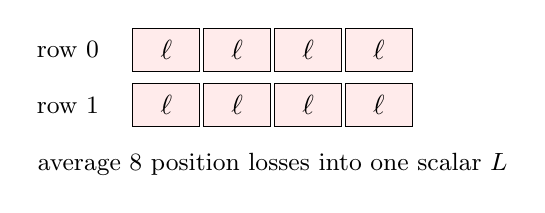
\begin{tikzpicture}[
  cell/.style={draw, minimum width=0.85cm, minimum height=0.55cm, align=center},
  lab/.style={font=\small}
]
\node[lab] at (-1.25,0) {row 0};
\node[lab] at (-1.25,-0.7) {row 1};
\foreach \r in {0,1} {
  \foreach \c in {0,1,2,3} {
    \node[cell, fill=red!8] at (\c*0.9,-\r*0.7) {\(\ell\)};
  }
}
\node[lab] at (1.35,-1.45) {average 8 position losses into one scalar \(L\)};
\end{tikzpicture}
\end{center}

\term{Code logic}: flatten the first two axes, because cross entropy sees a table of predictions.

\begin{lstlisting}[language=Python]
# logits:  [B, T, V] = [2, 4, 9]
# targets: [B, T]    = [2, 4]
loss = F.cross_entropy(
    logits.view(B * T, V),  # [8, 9]
    targets.view(B * T),    # [8]
)
\end{lstlisting}

The flattening operation can be visualized as unrolling a grid of position predictions into a list:

\begin{center}
\begin{tikzpicture}[
  cell/.style={draw, minimum width=0.65cm, minimum height=0.5cm, align=center},
  arrow/.style={-{Latex[length=2mm]}, thick},
  lab/.style={font=\small}
]
\node[lab] at (1.2,0.8) {logits before loss: \shape{[2,4,9]}};
\foreach \r in {0,1} {
  \foreach \c in {0,1,2,3} {
    \node[cell, fill=blue!6] at (\c*0.72,-\r*0.6) {};
    \node[cell, fill=red!6] at (\c*0.72+0.08,-\r*0.6+0.08) {};
  }
}
\draw[arrow] (3.3,-0.3) -- (4.25,-0.3);
\node[lab] at (6.1,0.8) {flattened for cross entropy: \shape{[8,9]}};
\foreach \r in {0,1,2,3,4,5,6,7} {
  \node[cell, fill=red!8] at (5.0,-\r*0.35) {};
  \node[lab] at (5.75,-\r*0.35) {\scriptsize one 9-class prediction};
}
\node[lab, align=center] at (3.2,-3.0) {The math is unchanged. Only the memory view changes.};
\end{tikzpicture}
\end{center}

Targets flatten the same way:

\[
\shape{[2,4]} \rightarrow \shape{[8]}.
\]

Each flattened target chooses the correct class for the matching flattened logit row.

\section{Operation Gallery: Shape Changes In TinyGPT}

This gallery summarizes the visual logic of the main operations introduced so far.

\begin{longtable}{p{0.2\textwidth}p{0.26\textwidth}p{0.34\textwidth}}
\toprule
\term{Operation} & \term{Shape change} & \term{Meaning} \\
\midrule
Embedding lookup & \shape{[B,T]} \(\rightarrow\) \shape{[B,T,C]} & replace each ID with a vector \\
Position add & \shape{[B,T,C]} + \shape{[T,C]} & add order information to every batch row \\
Linear head & \shape{[B,T,C]} \(\rightarrow\) \shape{[B,T,V]} & score every vocabulary token \\
Softmax & \shape{[B,T,V]} \(\rightarrow\) \shape{[B,T,V]} & convert scores to probabilities \\
Loss flatten & \shape{[B,T,V]} \(\rightarrow\) \shape{[BT,V]} & make one row per prediction \\
Cross entropy & \shape{[BT,V]}, \shape{[BT]} \(\rightarrow\) scalar & average prediction penalty \\
\bottomrule
\end{longtable}

\begin{center}
\begin{tikzpicture}[
  box/.style={draw, rounded corners=2pt, minimum height=0.7cm, text width=2.2cm, align=center},
  arrow/.style={-{Latex[length=2mm]}, thick}
]
\node[box, fill=blue!5] (a) at (0,0) {IDs\\\shape{[2,4]}};
\node[box, fill=blue!5] (b) at (2.8,0) {embeddings\\\shape{[2,4,6]}};
\node[box, fill=blue!5] (c) at (5.6,0) {hidden states\\\shape{[2,4,6]}};
\node[box, fill=red!8] (d) at (8.4,0) {logits\\\shape{[2,4,9]}};
\node[box, fill=red!8] (e) at (8.4,-1.35) {flat logits\\\shape{[8,9]}};
\node[box, fill=red!8] (f) at (5.6,-1.35) {loss\\scalar};
\draw[arrow] (a) -- node[above] {\scriptsize lookup} (b);
\draw[arrow] (b) -- node[above] {\scriptsize blocks} (c);
\draw[arrow] (c) -- node[above] {\scriptsize linear} (d);
\draw[arrow] (d) -- node[right] {\scriptsize view} (e);
\draw[arrow] (e) -- node[below] {\scriptsize cross entropy} (f);
\end{tikzpicture}
\end{center}

\section{Perplexity}

Perplexity is:

\[
\operatorname{PPL} = e^L.
\]

If validation loss is \(L=2.0\), then:

\[
\operatorname{PPL}=e^2 \approx 7.39.
\]

A rough intuition is that the model is about as uncertain as choosing among 7 or 8 plausible tokens on average. This is only an approximation, but it is useful for reading language-model logs.

\section{Functions And Parameters}

A neural network is a parameterized function:

\[
f_\theta(x)=Z.
\]

For TinyGPT:

\begin{itemize}
  \item \(x\): token IDs with shape \shape{[2,4]};
  \item \(\theta\): all model parameters;
  \item \(Z\): logits with shape \shape{[2,4,9]}.
\end{itemize}

The parameters \(\theta\) include:

\begin{lstlisting}
token embedding table
position embedding table
attention projection matrices
MLP matrices
LayerNorm weights
output head weights
\end{lstlisting}

\begin{center}
\begin{tikzpicture}[
  box/.style={draw, rounded corners=2pt, minimum height=0.7cm, text width=2.3cm, align=center},
  arrow/.style={-{Latex[length=2mm]}, thick}
]
\node[box, fill=blue!5] (x) at (0,0) {input \(x\)\\\shape{[2,4]}};
\node[box, fill=blue!5] (theta) at (3.0,0) {parameters\\\(\theta\)};
\node[box, fill=red!8] (f) at (6.0,0) {TinyGPT\\\(f_\theta\)};
\node[box, fill=red!8] (z) at (9.0,0) {logits \(Z\)\\\shape{[2,4,9]}};
\draw[arrow] (x) -- (f);
\draw[arrow] (theta) -- (f);
\draw[arrow] (f) -- (z);
\end{tikzpicture}
\end{center}

Training solves:

\[
\theta^\star = \arg\min_{\theta} L(\theta).
\]

In words: find parameter values that make the loss small.

\section{Derivatives And Gradients}

A derivative tells how a function changes when an input changes. A gradient is the multi-parameter version of this idea.

For TinyGPT, the loss \(L\) depends on many parameters. The gradient is:

\[
\nabla_\theta L =
\begin{bmatrix}
\frac{\partial L}{\partial \theta_1}\\
\frac{\partial L}{\partial \theta_2}\\
\vdots\\
\frac{\partial L}{\partial \theta_n}
\end{bmatrix}.
\]

Each entry asks:

\begin{quote}
If this parameter changes a tiny bit, how does the loss change?
\end{quote}

Gradient descent updates parameters by moving opposite the gradient:

\[
\theta_{\text{new}} =
\theta_{\text{old}} - \eta \nabla_\theta L.
\]

If a parameter change would increase loss, the update moves the other way.

\begin{center}
\begin{tikzpicture}[
  axis/.style={->, thick},
  arrow/.style={-{Latex[length=2mm]}, thick},
  dot/.style={circle, fill=red!70, inner sep=2pt}
]
\draw[axis] (-0.3,0) -- (7,0) node[right] {parameter value};
\draw[axis] (0,-0.2) -- (0,3.2) node[above] {loss};
\draw[thick, blue!60!black, domain=0.4:6.4, samples=80] plot (\x,{0.28*(\x-3.5)^2+0.5});
\node[dot] (p) at (5.3,{0.28*(5.3-3.5)^2+0.5}) {};
\draw[arrow, red!70!black] (p) -- ++(-1.0,-0.45);
\node[font=\small, align=center] at (5.5,2.35) {move opposite\\the gradient};
\end{tikzpicture}
\end{center}

\term{Code logic}: after \texttt{loss.backward()}, each trainable tensor has a \texttt{.grad} field.

\begin{lstlisting}[language=Python]
logits, loss = model(x, y)
loss.backward()

for name, param in model.named_parameters():
    print(name, param.shape, param.grad.shape)
\end{lstlisting}

\section{Why Backpropagation Works}

TinyGPT is a composition of functions:

\[
x
\rightarrow
\text{embeddings}
\rightarrow
\text{Transformer blocks}
\rightarrow
\text{logits}
\rightarrow
\text{loss}.
\]

Mathematically:

\[
L(x) = \ell(g_4(g_3(g_2(g_1(x))))).
\]

Backpropagation applies the chain rule through this composition. If

\[
z=g(y),\qquad y=h(x),
\]

then:

\[
\frac{dz}{dx} =
\frac{dz}{dy}
\frac{dy}{dx}.
\]

The practical meaning is:

\begin{quote}
The loss sends a learning signal backward through every operation that helped produce it.
\end{quote}

\begin{center}
\begin{tikzpicture}[
  box/.style={draw, rounded corners=2pt, minimum height=0.68cm, text width=2.0cm, align=center},
  fwd/.style={-{Latex[length=2mm]}, thick, blue!60!black},
  bwd/.style={-{Latex[length=2mm]}, thick, red!70!black}
]
\node[box, fill=blue!5] (x) at (0,0) {IDs};
\node[box, fill=blue!5] (e) at (2.3,0) {embeddings};
\node[box, fill=blue!5] (m) at (4.6,0) {model};
\node[box, fill=blue!5] (z) at (6.9,0) {logits};
\node[box, fill=red!8] (l) at (9.2,0) {loss};
\draw[fwd] (x) -- (e);
\draw[fwd] (e) -- (m);
\draw[fwd] (m) -- (z);
\draw[fwd] (z) -- (l);
\draw[bwd] (l.south) .. controls (7.5,-1.2) and (5.5,-1.2) .. (m.south);
\draw[bwd] (m.south) .. controls (3.3,-1.2) and (2.6,-1.2) .. (e.south);
\node[font=\small, text=blue!60!black] at (4.6,0.72) {forward values};
\node[font=\small, text=red!70!black] at (4.6,-1.45) {backward gradients};
\end{tikzpicture}
\end{center}

\section{Math-To-Code Reference}

The following reference table is meant to make source code less mysterious.

\begin{longtable}{p{0.23\textwidth}p{0.24\textwidth}p{0.35\textwidth}}
\toprule
\term{Math} & \term{PyTorch idea} & \term{TinyGPT example} \\
\midrule
\(\mathbf{v}\in\mathbb{R}^{6}\) & rank-1 tensor & one token embedding \\
\(W\in\mathbb{R}^{6\times9}\) & rank-2 tensor & output head weight \\
\(X\in\mathbb{R}^{2\times4\times6}\) & rank-3 tensor & embedded batch \\
\(XW+b\) & \texttt{nn.Linear} & hidden to logits \\
\(\operatorname{softmax}(z)\) & \texttt{torch.softmax} & logits to probabilities \\
\(-\log p_y\) & cross entropy & loss for correct token \\
\(\nabla_\theta L\) & \texttt{param.grad} & parameter update signal \\
\(\theta-\eta\nabla L\) & optimizer step & improve weights \\
\bottomrule
\end{longtable}

\engineering

Before implementing any layer, write a four-line contract:

\begin{lstlisting}
input shape:
parameter shape:
output shape:
meaning of each axis:
\end{lstlisting}

For example, the output head contract is:

\begin{lstlisting}
input shape:      [B, T, C] = [2, 4, 6]
parameter shape:  [C, V]    = [6, 9]
output shape:     [B, T, V] = [2, 4, 9]
meaning:          one vocabulary score vector per position
\end{lstlisting}

Most early LLM bugs are not deep mysteries. They are shape bugs, dtype bugs, device bugs, indexing bugs, or mismatches between tokenizer and model configuration.

\labtitle{Manual Softmax And Loss}

Suppose TinyGPT has seen:

\begin{quote}
\texttt{Tiny GPT models learn from}
\end{quote}

and the next token should be \texttt{tokens}, ID \(7\). For a simplified three-token vocabulary slice, suppose the logits are:

\[
\mathbf{z} = [2.0,1.0,0.0],
\]

where index \(0\) is the correct class in the slice.

\begin{enumerate}
  \item Compute the softmax probabilities.
  \item Compute the negative log likelihood loss if the correct class is index \(0\).
  \item Compute the loss if the correct class is index \(2\).
  \item Explain which target produces the larger loss and why.
\end{enumerate}

\section{Chapter Questions}

\begin{enumerate}
  \item In TinyGPT, what does \(V=9\) mean?
  \item What is the difference between a token ID and an embedding vector?
  \item If \(B=2\), \(T=4\), and \(C=6\), what is the shape after token embedding?
  \item What shape does the output head produce if \(V=9\)?
  \item Why are logits not probabilities?
  \item What two properties must a probability distribution satisfy?
  \item Why does cross entropy use \(-\log p_y\)?
  \item Why does batch loss average over \(B\times T\) predictions?
  \item What does the gradient \(\nabla_\theta L\) tell the optimizer?
  \item Why is backpropagation connected to the chain rule?
\end{enumerate}

\section{Solutions}

\begin{enumerate}
  \item \(V=9\) means the TinyGPT vocabulary contains nine possible token IDs, \(0\) through \(8\). At each position, the model outputs nine logits.

  \item A token ID is a discrete index, such as \(2\) for \texttt{Tiny}. An embedding vector is a learned list of numbers, such as a vector in \(\mathbb{R}^{6}\), that represents the token numerically.

  \item The shape after token embedding is \shape{[2,4,6]}. There are two examples, four positions, and six embedding features per token.

  \item The output head produces \shape{[2,4,9]}. Each of the eight positions has nine vocabulary scores.

  \item Logits are raw scores. They may be negative, positive, or any real number. Probabilities must be nonnegative and sum to one, so logits need softmax first.

  \item A probability distribution must satisfy \(p_i\geq 0\) for every \(i\), and \(\sum_i p_i=1\).

  \item Cross entropy uses \(-\log p_y\) because it gives low loss when the correct token probability is high and high loss when the correct token probability is low.

  \item A batch with shape \shape{[B,T]} contains one prediction target at every position of every example. Therefore there are \(B\times T\) position losses to average.

  \item The gradient tells the optimizer how the loss changes with respect to each parameter. The optimizer uses it to adjust parameters in a direction that tends to reduce loss.

  \item Backpropagation is the chain rule applied efficiently through a computation graph. Since TinyGPT is a composition of functions, the chain rule tells how loss gradients flow backward through all operations.
\end{enumerate}

\section{Lab Solution}

For:

\[
\mathbf{z}=[2.0,1.0,0.0],
\]

compute exponentials:

\[
e^2\approx7.389,\qquad e^1\approx2.718,\qquad e^0=1.
\]

The denominator is:

\[
7.389+2.718+1=11.107.
\]

So the softmax probabilities are approximately:

\[
\left[
\frac{7.389}{11.107},
\frac{2.718}{11.107},
\frac{1}{11.107}
\right]
=
[0.665,0.245,0.090].
\]

If the correct class is index \(0\):

\[
L=-\log(0.665)\approx0.408.
\]

If the correct class is index \(2\):

\[
L=-\log(0.090)\approx2.408.
\]

The second loss is larger because the model assigned only about \(9\%\) probability to class \(2\). Cross entropy punishes the model when it gives low probability to the correct answer.
